\chapter{Lezione 5}
\label{chap:lezione_05} 

\begin{flushright}
\textit{Data: 15/10/2025}
\end{flushright}

% Comandi personalizzati
\newcommand{\deriv}[2]{\frac{d #1}{d #2}}
\newcommand{\pderiv}[2]{\frac{\partial #1}{\partial #2}}


\section{Introduzione allo Scaling e Leggi di Potenza}

In questa lezione si affrontano i concetti di variabili di scaling, leggi di potenza e modelli generativi. Sebbene nelle lezioni precedenti siano stati introdotti strumenti per trattare le distribuzioni a coda lunga (long-tails) e le leggi di potenza, non è stata ancora fornita una spiegazione teorica fondamentale sul \textit{perché} tali distribuzioni siano così ubiquitarie in natura.

\subsection{Argomentazioni di Galileo sullo Scaling}
Il concetto di scaling non è recente; Galileo Galilei si interrogava su queste problematiche in modo molto concreto, analizzando le dimensioni delle ossa negli animali (si veda il "Dialogo sopra i due massimi sistemi del mondo").

Consideriamo la relazione tra lunghezza caratteristica $L$, massa $M$ e resistenza strutturale $S$ (Strength).
Se scaliamo la dimensione lineare di un oggetto di un fattore (ad esempio raddoppiandola):
\begin{equation}
    L \to 2L \implies M \propto L^3 \to 8M
\end{equation}
La massa scala con il cubo della lunghezza (assumendo densità costante). Tuttavia, la resistenza di un osso dipende dalla sua sezione trasversale $A \propto R^2$ (dove $R$ è il raggio o diametro dell'osso):
\begin{equation}
    S \propto R^2 \quad (\text{o } D^2)
\end{equation}
Se scaliamo geometricamente l'animale mantenendo le proporzioni ($R \propto L$):
\begin{equation}
    S \to 4S
\end{equation}
Si crea una discrepanza: il peso aumenta di un fattore 8, ma la capacità di sostenerlo aumenta solo di un fattore 4.
\begin{equation}
    \frac{\text{Peso}}{\text{Resistenza}} \propto \frac{L^3}{L^2} = L
\end{equation}
Questa è la ragione per cui non possono esistere giganti geometricamente simili agli umani: le loro ossa cederebbero sotto il proprio peso. Affinché la struttura regga (ovvero, per mantenere costante lo stress $S/M \approx cost$), la sezione dell'osso dovrebbe scalare come la massa:
\begin{equation}
    R^2 \sim M \sim L^3 \implies R \sim L^{3/2}
\end{equation}
Le ossa dovrebbero quindi diventare sproporzionatamente grosse rispetto alla lunghezza.
Galileo fornì una prova sperimentale utilizzando due lenze da pesca con diametri $d_1$ e $d_2$. Verificò che il rapporto del carico di rottura corrispondeva esattamente al rapporto dei quadrati dei diametri:
\begin{equation}
    \frac{S_1}{S_2} = \frac{d_1^2}{d_2^2}
\end{equation}

\subsection{Scaling in Biologia: Relazioni Allometriche}
In biologia, le leggi di scaling sono onnipresenti e prendono il nome di \textbf{Relazioni Allometriche}. Assumono la forma generale:
\begin{equation}
    Y = Y_0 M^b
\end{equation}
dove $Y$ è una variabile biologica e $M$ è la massa.
\begin{itemize}
    \item \textbf{Legge di Kleiber:} Il metabolismo basale $B$ scala come $M^{3/4}$. Questo esponente $3/4$ (invece del $2/3$ geometrico superficiale) si applica sorprendentemente anche a interi ecosistemi.
    \item \textbf{Circolazione:} Il tempo di circolazione sanguigna scala come $T \sim M^{1/4}$.
    \item \textbf{Frequenza cardiaca:} Scala con esponente negativo $\omega \sim M^{-1/4}$. Il cuore di un elefante batte molto più lentamente di quello di un topo.
\end{itemize}
Esistono dibattiti teorici aperti sull'origine esatta della legge dei $3/4$ (si vedano i lavori di West, Brown, Enquist). È cruciale distinguere tra il dato empirico misurato e la teoria ("la lente") usata per interpretarlo.

\subsection{Scaling nei Sistemi Sociali}
Nei sistemi sociali e urbani, osserviamo diverse classi di scaling rispetto alla popolazione $N$:
\begin{equation}
    Y \sim N^{\beta}
\end{equation}
\begin{itemize}
    \item \textbf{$\beta > 1$ (Superlineare):} Quantità legate all'interazione sociale (innovazione, brevetti, crimine). Qui "$1+1 > 2$".
    \item \textbf{$\beta \approx 1$ (Lineare):} Quantità legate ai bisogni individuali (es. numero di case).
    \item \textbf{$\beta < 1$ (Sublineare):} Infrastrutture (strade, reti elettriche). Ottimizzazione e economie di scala.
\end{itemize}

\section{Derivazione della Legge di Potenza dallo Scaling}

Un modello generativo deve spiegare perché queste leggi emergono. Partiamo dall'ipotesi di invarianza di scala per una distribuzione di probabilità $P(x)$.
La relazione di scaling impone che riscalando la variabile $x$ di un fattore $\lambda$, la distribuzione rimanga la stessa a meno di un pre-fattore:
\begin{equation}
    P(\lambda x) = g(\lambda) P(x)
\end{equation}
Vogliamo determinare la forma funzionale di $P(x)$.
Per $x=1$, l'equazione diventa $P(\lambda) = g(\lambda)P(1)$, da cui ricaviamo la funzione di scaling:
\begin{equation}
    g(\lambda) = \frac{P(\lambda)}{P(1)}
\end{equation}
Sostituendo nell'equazione originale:
\begin{equation}
    P(\lambda x) = \frac{P(\lambda)}{P(1)} P(x)
\end{equation}
Differenziamo entrambi i membri rispetto a $\lambda$:
\begin{equation}
    \pderiv{}{\lambda} P(\lambda x) = \frac{P(x)}{P(1)} \deriv{P(\lambda)}{\lambda}
\end{equation}
Applicando la regola della catena a sinistra ($y=\lambda x \to dy/d\lambda = x$):
\begin{equation}
    x P'(\lambda x) = \frac{P(x)}{P(1)} P'(\lambda)
\end{equation}
Poniamo ora $\lambda = 1$:
\begin{equation}
    x P'(x) = \frac{P'(1)}{P(1)} P(x)
\end{equation}
Il termine $\frac{P'(1)}{P(1)}$ è una costante. Definiamola come $-\beta$.
Otteniamo l'equazione differenziale:
\begin{equation}
    \frac{P'(x)}{P(x)} = -\frac{\beta}{x} \implies \deriv{(\ln P)}{x} = -\frac{\beta}{x}
\end{equation}
Integrando:
\begin{tcolorbox}[colback=yellow!25, colframe=yellow!75!orange, coltitle=black, title=\textbf{Legge di Potenza}]
\begin{equation}
    P(x) = P(0) x^{-\beta}
\end{equation}
L'invarianza di scala (o "zoom-in/zoom-out invariance") implica necessariamente una distribuzione a legge di potenza (scale-free).
\end{tcolorbox}

\section{Combinazione di Esponenziali}

Analizziamo un primo modello generativo ("toy model") che ottiene una legge di potenza combinando distribuzioni esponenziali.
Sia $X$ una variabile casuale con distribuzione esponenziale:
\begin{equation}
    \rho_X(x) = c_1 e^{ax}
\end{equation}
Definiamo una nuova variabile $Y$ attraverso una trasformazione esponenziale:
\begin{equation}
    Y = c_2 e^{bX}
\end{equation}
Vogliamo trovare la distribuzione $\tilde{\rho}(y)$.
Invertiamo la relazione:
\begin{equation}
    \frac{Y}{c_2} = e^{bX} \implies bX = \ln\left(\frac{Y}{c_2}\right) \implies X = \frac{1}{b} \ln\left(\frac{Y}{c_2}\right)
\end{equation}
Usiamo la conservazione della probabilità: $\tilde{\rho}(y) dy = \rho_X(x) dx$.
Calcoliamo lo Jacobiano della trasformazione inversa:
\begin{equation}
    \frac{dX}{dY} = \frac{d}{dY} \left[ \frac{1}{b} (\ln Y - \ln c_2) \right] = \frac{1}{bY}
\end{equation}
Sostituiamo nella formula:
\begin{equation}
    \tilde{\rho}(y) = \rho_X(X(y)) \left| \frac{dX}{dY} \right| = c_1 e^{a \left[ \frac{1}{b} \ln\left(\frac{y}{c_2}\right) \right]} \cdot \frac{1}{bY}
\end{equation}
Definiamo $K = c_1/b$. Manipoliamo il termine esponenziale:
\begin{equation}
    e^{\ln\left( (y/c_2)^{a/b} \right)} = \left( \frac{y}{c_2} \right)^{\frac{a}{b}} \propto y^{\frac{a}{b}}
\end{equation}
Quindi:
\begin{equation}
    \tilde{\rho}(y) = K y^{\frac{a}{b}} \cdot y^{-1} = K y^{\frac{a}{b} - 1} = K y^{-\left(1 - \frac{a}{b}\right)}
\end{equation}
Abbiamo ottenuto una legge di potenza $P(y) \sim y^{-\beta}$ con esponente $\beta = 1 - \frac{a}{b}$.

\section{Monkey Typewriter}
Sia $m$ il numero di caratteri distinti disponibili (es. 26 lettere).
Sia $p$ la probabilità di premere la barra spaziatrice (generazione di un fine parola).
La probabilità di premere un qualsiasi altro tasto specifico è $p_l = \frac{1-p}{m}$. Una parola di lunghezza $S$ è composta da $S$ caratteri specifici seguiti da uno spazio. Poiché l'ordine conta (le lettere sono fissate), la probabilità di generare una \textit{specifica} parola di lunghezza $S$ è:
\begin{equation}
    P(\text{word}_S) = \left( \frac{1-p}{m} \right)^S \cdot p
\end{equation}
Possiamo riscrivere questa probabilità come un esponenziale della lunghezza:
\begin{equation}
    P(\text{word}_S) = p \cdot e^{S \ln\left(\frac{1-p}{m}\right)} = p \cdot  e^{bS}
\end{equation}
con $b = \ln\left(\frac{1-p}{m}\right) < 0$.


Dunque, questo significa che più lunga è la parola, minore è la sua probabilità, dato che $b < 0$. In altre parole, la distribuzione delle lunghezze delle parole decade esponenzialmente. Tuttavia, per ogni lunghezza $S$ ci sono $m^S$ possibili combinazioni distinte di lettere, quindi il \textit{numero di parole} di tale lunghezza cresce esponenzialmente con $S$. Abbiamo pertanto due esponenziali opposti: uno decrescente (la probabilità di ogni sequenza) e uno crescente (il numero di sequenze possibili).

\subsection{Relazione Rango-Frequenza}
Vogliamo trovare la relazione tra la frequenza della parola (probabilità) e il suo rango $r$ (classifica dalla più frequente alla meno frequente).
Il numero totale di parole possibili con lunghezza $\le S$ determina il rango massimo associato alla lunghezza $S$.
Somma della serie geometrica delle parole possibili (m parole lunghe 1, $m^2$ lunghe 2, ...):
\begin{equation}
    r(S) \approx \sum_{i=1}^{S} m^i = \frac{m^{S+1}-m}{m-1} \approx \frac{m^{S+1}}{m-1} \approx m^S
\end{equation}
Invertendo per grandi $S$:
\begin{equation}
    S \approx \log_m r
\end{equation}
Sostituiamo $S$ nell'espressione della probabilità (frequenza $f(r)$):
\begin{equation}
    f(r) \sim \left( \frac{1-p}{m} \right)^{\log_m r}
\end{equation}
Usiamo l'identità $x^{\log_m r} = r^{\log_m x}$:
\begin{equation}
    f(r) \sim r^{\log_m \left( \frac{1-p}{m} \right)} = r^{\log_m(1-p) - \log_m m} = r^{\log_m(1-p) - 1}
\end{equation}
Questa è la Legge di Zipf $f(r) \sim r^{-\alpha}$ con esponente:
\begin{equation}
    \alpha = 1 - \log_m(1-p)
\end{equation}
Pertanto, anche questo processo puramente casuale, una ``scimmia'' che digita casualmente lettere e spazi, produce una \textit{distribuzione a legge di potenza} nella relazione rango-frequenza delle parole. 

Inserendo valori reali ($m=26, p \approx 0.2$), si ottiene $\alpha \approx 1.01$, che è sorprendentemente vicino al valore reale della legge di Zipf ($\alpha \approx 1$).
Tuttavia, il modello è concettualmente errato per il linguaggio umano (eccetto forse le lingue agglutinanti), poiché prevede che le parole più corte siano sempre le più frequenti in modo monotono, mentre i dati reali mostrano una distribuzione log-normale o simile per le lunghezze.
Più in generale, tutto ciò a cui applichiamo solitamente le combinazioni di esponenziali finisce per funzionare in un intervallo molto specifico prima che sia necessario considerare qualche tipo di correzione empirica.

\begin{figure}[h]
\centering
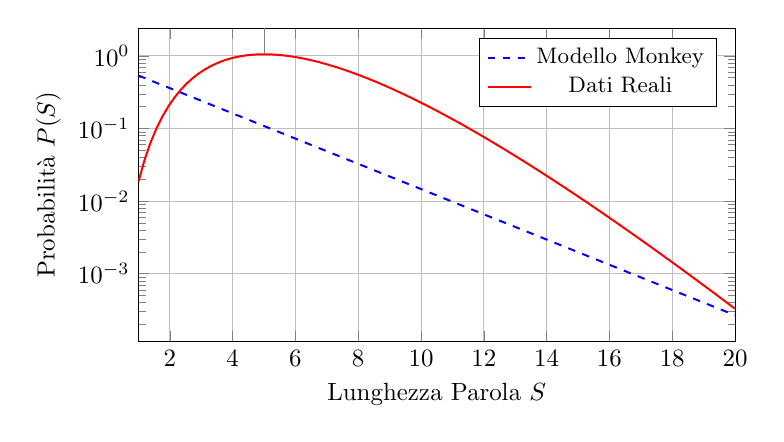
\begin{tikzpicture}[scale=0.9]
    \begin{axis}[
        width=10cm, height=6cm,
        xlabel={Lunghezza Parola $S$},
        ylabel={Probabilità $P(S)$},
        ymode=log,
        domain=1:20, % Partiamo da 1, S=0 non ha senso fisico
        xmin=1, xmax=20,
        legend pos=north east, % Spesso copre meno dati in alto a destra o sud-ovest
        grid=major,
        samples=100 % Aumentato per curve più morbide
    ]
    
    % Modello Monkey: Decadimento esponenziale puro
    % P(S) ~ exp(-bS). Normalizzato a occhio per il grafico.
    \addplot[blue, thick, dashed] {0.8*exp(-0.4*x)};
    \addlegendentry{\small Modello Monkey}

    % Realtà: Distribuzione Gamma/Lognormale
    % x^alpha * exp(-beta*x). Picco a x = alpha/beta.
    % Se alpha=5 e beta=1, picco a 5.
    \addplot[red, thick] {0.05 * x^5 * exp(-1*x)}; 
    \addlegendentry{\small Dati Reali}
    
    % Annotazione
    \node[coordinate, pin=above:{Picco tipico ($\sim 5$ chars)}] at (axis cs: 5, 0.05 * 3125 * 0.0067) {};
    
    \end{axis}
\end{tikzpicture}
\caption{Confronto tra la previsione teorica e la distribuzione reale della lunghezza delle parole.}
\end{figure}

\section{Inversione dei Quantili}

Sebbene si tratti di un passaggio elementare, è opportuno esaminarlo; essenzialmente, partendo da un processo di tipo legge di potenza (\textit{power law}), si osserverà conseguentemente una legge di potenza. Si consideri una variabile stocastica distribuita secondo $\rho(y)$ e una variabile stocastica derivata $x$ tale che $x = 1/y$. Si ha:

\begin{equation}
    \tilde{\rho}(x) = \rho(y) \left| \frac{dy}{dx} \right| = \rho\left(\frac{1}{x}\right) \frac{1}{x^2} \xrightarrow[x \gg 1]{y \ll 1} \rho(0) x^{-2} \sim x^{-2}.
    \label{eq:quantile_inversion}
\end{equation}

Di conseguenza, indipendentemente dalla distribuzione della variabile $y$, il comportamento asintotico della coda segue una legge di potenza. Ad esempio, nel modello di Ising, analizzando le fluttuazioni della magnetizzazione attorno alla media, definite come $\delta = \Delta m$, si osserva che $\delta \sim m^{-1}$, da cui ne deriva che $\rho(\delta) \sim m^{-2}$ nelle code della distribuzione.

\section{Processo di Yule-Simon}
Dedicheremo un'analisi approfondita a questo modello generativo di leggi di potenza, dato il suo notevole interesse teorico e la sua vasta applicabilità nei processi di innovazione: dalla biologia alla generazione del linguaggio e, più in generale, nella modellizzazione della frequenza con cui l'innovazione emerge nelle dinamiche sociali. Tali caratteristiche rendono questo modello uno standard di riferimento per la generazione di distribuzioni a coda pesante (\textit{heavy-tailed}).

Il modello giustifica un comportamento osservato in una molteplicità di sistemi, noto informalmente come \textbf{Rich-Get-Richer}  o \textbf{Preferential Attachment}. Ad esempio, nella distribuzione delle specie, è ragionevole attendersi che le specie più antiche siano anche le più diffuse. Il medesimo principio si applica a numerosi altri domini: parole già frequenti tendono ad apparire con frequenza ancora maggiore, articoli scientifici già citati hanno una maggiore probabilità di ricevere ulteriori citazioni...

In sintesi, il modello Yule–Simon fornisce il fondamento matematico per questo processo di auto-rinforzo, in cui la probabilità di acquisire nuovi membri (o occorrenze) cresce in funzione del numero già accumulato. Questa dinamica conduce naturalmente a distribuzioni a coda pesante (simili a leggi di potenza), dove un numero esiguo di entità domina il sistema, mentre la maggioranza rimane rara.


\subsubsection*{Il Processo di Yule (1922)}
Sebbene l'analisi di Simon sia successiva di circa trent'anni, è Yule a definire le dinamiche fondamentali del processo. Originariamente formulato in ambito biologico, introdurremo qui i postulati utilizzando la terminologia linguistica. Le regole generali che governano il processo sono le seguenti:

\begin{itemize}
    \item Nuove specie possono emergere nel sistema, ma non possono estinguersi.
    \item Una categoria (o genere, in senso biologico) a cui sono associate $k$ specie, acquisisce nuove specie con un tasso proporzionale al numero di specie già possedute (meccanismo \textit{rich-get-richer}).
    \item Occasionalmente, una parola diverge talmente da un'altra, o una mutazione apporta variazioni così significative, che la nuova specie non risulta classificabile nel genere di origine, determinando così la creazione di un nuovo genere o di una nuova categoria.
\end{itemize}

\noindent Mentre i principi sono attribuiti a Yule, lo sviluppo formale del processo è ascritto a Simon (1955). 

\subsubsection{Definizione e Master Equation}

Si consideri lo stato iniziale al tempo $t = 0$: il sistema è costituito da un singolo elemento (una parola in un dizionario o una specie in un genere). Ad ogni passo temporale $t \to t + 1$, viene aggiunto una nuova specie secondo le seguenti regole. Se definiamo $E(t)$ come l'evento di assegnazione al tempo $t$:

\begin{equation}
    E(t+1) = 
    \begin{cases} 
    \text{Raggruppato in un nuovo genere} & \text{Prob} = p \\
    \text{Raggruppato in un genere preesistente} & \text{Prob} = 1-p 
    \end{cases}
    \label{eq:assignment_prob}
\end{equation}

Si osservi che, indipendentemente dall'esito, un nuovo elemento viene introdotto nel sistema; la questione dirimente è se tale elemento costituisca un nuovo genere o se vada ad accrescere un genere preesistente.
Sia $D(t)$ il numero di generi distinti presenti al tempo $t$. Poiché la probabilità di apparizione di un nuovo genere è $p$, ci attendiamo che il tasso di variazione di $D(t)$ sia pari a $p$:

\begin{equation}
    \frac{d}{dt}D(t) = p \implies D(t) = D_{0} + p t.
\end{equation}
Si nota una dipendenza lineare in $t$, analoga alla legge di Heaps.


\noindent Ci interroghiamo ora sulla distribuzione del numero di generi aventi $k$ specie al tempo $t$, denotata come $P_{k,t}$. Per determinare tale quantità, utilizzeremo il formalismo della \textbf{Master Equation}, combinato con l'approssimazione al continuo. Nel passaggio temporale $t \to t+1$, l'aggiunta di una nuova parola (o specie) può comportare una delle seguenti tre transizioni per la variabile $P_{k,t}$:

\begin{enumerate}
    \item Un genere con $k-1$ specie acquisisce una nuova specie, incrementando il contatore $P_{k,t}$ di un'unità.
    \item Un genere con $k$ specie acquisisce una nuova specie (diventando un genere con $k+1$ specie), decrementando il contatore $P_{k,t}$ di un'unità.
    \item Un nuovo genere appare con una singola specie, incrementando il contatore $P_{1,t}$ (questo termine influenza solo il caso $k=1$).
\end{enumerate}

\noindent Formalizziamo matematicamente questi contributi. Ricordando che il fattore $(1-p)$ funge da selettore per l'assegnazione a generi esistenti, il termine di transizione è dato da:

\begin{equation}
\Delta P =    \underbrace{(1-p) \frac{(k-1)P_{k-1,t}}{t}}_{\text{Caso 1}} - \underbrace{(1-p) \frac{k P_{k,t}}{t}}_{\text{Caso 2}} + \underbrace{p \delta_{k,1}}_{\text{Caso 3}}
\end{equation}

\noindent Analizziamo i termini: nel Caso 1, dato che il sistema contiene $t$ specie totali al tempo $t$, e assumendo il meccanismo di attaccamento preferenziale, la probabilità che la nuova specie sia assegnata a un genere specifico di dimensione $k-1$ è proporzionale a $(k-1)/t$. Poiché vi sono $P_{k-1,t}$ generi di tale dimensione, il contributo totale è:

\begin{equation}
    \frac{k-1}{t} P_{k-1,t}.
\end{equation}
Applicando il medesimo ragionamento al Caso 2 e considerando il termine sorgente del Caso 3, otteniamo la Master Equation completa:

\begin{equation}
    P_{k,t+1} = P_{k,t} + (1-p)\frac{(k-1)P_{k-1,t}}{t} - (1-p)\frac{k P_{k,t}}{t} + p \delta_{k,1}.
\end{equation}
Possiamo riordinare i termini per evidenziare la differenza finita temporale:

\begin{equation}
    P_{k,t+1} - P_{k,t} = \frac{(1-p)}{t} \left[ (k-1)P_{k-1,t} - k P_{k,t} \right] + p \delta_{k,1}.
\end{equation}

\subsubsection*{Limite del Continuo}

Applichiamo ora l'approssimazione al continuo per grandi $t$ e $k$:

\begin{equation}
    \begin{cases}
    P_{k,t+1} - P_{k,t} \simeq \frac{\partial P_{k}}{\partial t} \\
    P_{k,t} - P_{k-1,t} \simeq \frac{\partial P_{k}}{\partial k}
    \end{cases}
\end{equation}
Si noti che l'approssimazione della differenza finita rispetto a $k$ implica:
\begin{equation}
    \frac{\partial f(x)}{\partial x} \approx f(x) - f(x-1).
\end{equation}
Pertanto, il termine al lato destro dell'equazione può essere riscritto come una derivata rispetto a $k$:

\begin{equation}
    (k-1)P_{k-1,t} - k P_{k,t} \simeq - \frac{\partial (k P_{k,t})}{\partial k}.
\end{equation}
La Master Equation assume quindi la forma di un'equazione differenziale alle derivate parziali (dove la delta di Kronecker è trattata come una delta di Dirac):

\begin{equation}
    \frac{\partial P_{k,t}}{\partial t} = - \frac{(1-p)}{t} \frac{\partial (k P_{k,t})}{\partial k} + p \delta(k-1).
\end{equation}
Ipotizziamo che per $t \to \infty$ il rapporto $P_{k,t}/t$ tenda a una distribuzione stazionaria $q_k$, dipendente unicamente dal numero di specie. Effettuando la sostituzione $P_{k,t} = q_k t$, si ottiene:

\begin{equation}
    q_k = -(1-p)(q_k + k q_k') + p \delta(k-1) \implies (1-p) k q_k' = p \delta(k-1) - (2-p)q_k.
\end{equation}
Per risolvere l'equazione, consideriamo il dominio $k > 1$ (dove la delta è nulla):

\begin{equation}
    \frac{dq_k}{q_k} = - \frac{2-p}{1-p} \frac{dk}{k} \implies q_k = C k^{-\frac{2-p}{1-p}}.
\end{equation}
La costante $C$ viene determinata tramite la condizione di normalizzazione nell'intervallo $[1, \infty)$:

\begin{equation}
    C \int_{1}^{\infty} k^{-\alpha} dk = \left. \frac{C}{1-\alpha} k^{1-\alpha} \right|_{1}^{\infty} = 1.
\end{equation}
Dato che l'esponente $\alpha = \frac{2-p}{1-p}$ è strettamente maggiore di 1, l'integrale converge e si ottiene:

\begin{equation}
    C = \alpha - 1 = \frac{1}{1-p}.
\end{equation}
Pertanto, la distribuzione asintotica per $k \ge 1$ è:

\begin{equation}
    q_k = \frac{1}{1-p} k^{-\frac{2-p}{1-p}}.
\end{equation}
Possiamo esprimere il risultato come una legge di potenza $q_k \propto k^{-\alpha}$, con esponente:

\begin{equation}
    \alpha = \frac{2-p}{1-p} = 1 + \frac{1}{1-p}.
\end{equation}
Richiamando la relazione tra la funzione di densità di probabilità (PDF) e la legge di Zipf $f(R) \sim R^{-\gamma}$, con $\gamma = 1/(\alpha-1)$, otteniamo:

\begin{equation}
    \gamma = 1-p.
\end{equation}
Se la probabilità di introdurre un nuovo genere è molto piccola ($p \ll 1$), allora $\gamma \sim 1$. Questo risultato è coerente con le osservazioni empiriche di Zipf sui testi, dimostrando che il processo di Yule-Simon nello stato stazionario riproduce la legge di Zipf.

\subsection{Approccio Alternativo}

Esiste un metodo alternativo per giungere alla medesima conclusione, ponendosi in un contesto più realistico.
Sia $n_i(t)$ il numero di copie della $i$-esima parola al tempo $t$. Definiamo $p$ come la probabilità di generare una parola inedita e $1-p$ come la probabilità di generare una parola già osservata.
La frequenza relativa della parola $i$ al tempo $t$ è:

\begin{equation}
    f_i(t) = \frac{n_i(t)}{t}.
\end{equation}
Assumiamo l'\textit{ansatz} secondo cui il tasso di variazione del numero di occorrenze sia proporzionale alla frequenza stessa:

\begin{equation}
    \frac{d}{dt}n_i(t) = (1-p)\frac{n_i(t)}{t}.
\end{equation}
Integrando tra il tempo di prima apparizione $t_i$ (dove $n_i(t_i)=1$) e il tempo attuale $t$:

\begin{equation}
    \ln\left(\frac{n_i(t)}{1}\right) = (1-p) \ln\left(\frac{t}{t_i}\right) \implies n_i(t) = \left( \frac{t}{t_i} \right)^{1-p}.
\end{equation}
Per determinare la distribuzione di probabilità di $n_i$, passiamo attraverso la distribuzione cumulativa. Calcoliamo la probabilità che $n_i$ sia minore o uguale a un valore $n$:

\begin{equation}
    n_i(t) \le n \implies \left(\frac{t}{t_i}\right)^{1-p} \le n \implies t_i \ge t n^{-\frac{1}{1-p}} \equiv \tau.
\end{equation}
La probabilità $P(t_i \ge \tau)$ rappresenta la frazione di parole introdotte dopo il tempo $\tau$. Utilizzando la funzione $D(t)$ (numero di parole distinte) introdotta precedentemente:

\begin{equation}
    P(t_i \ge \tau) \approx 1 - \frac{D(\tau)}{D(t)} = 1 - \frac{N_0 + p\tau}{N_0 + pt}.
\end{equation}
Sostituendo $\tau$ e considerando il limite asintotico per grandi $t$ (trascurando $N_0$):

\begin{equation}
    P(n_i \le n) \approx 1 - \frac{p t n^{-\frac{1}{1-p}}}{p t} = 1 - n^{-\frac{1}{1-p}}.
\end{equation}
Infine, otteniamo la distribuzione di probabilità derivando la cumulativa rispetto a $n$:

\begin{equation}
    P(n) = \frac{d}{dn} P(n_i \le n) = \frac{1}{1-p} n^{-\frac{1}{1-p}-1} \sim n^{-\beta},
\end{equation}
con $\beta = 1 + \frac{1}{1-p}$, confermando esattamente il risultato ottenuto con la Master Equation.
